\documentclass[aspectratio=169]{beamer}

\usetheme{Boadilla}
\usefonttheme{professionalfonts}
\setbeamertemplate{navigation symbols}{}
\setbeamertemplate{itemize items}[circle]
\setbeamertemplate{enumerate items}[default]
\setbeamertemplate{headline}{}

\usepackage[utf8]{inputenc}
\usepackage[T1]{fontenc}
\usepackage{lmodern}
\usepackage{amsmath}
\usepackage{booktabs}
\usepackage{tabularx}
\usepackage{array}
\usepackage{hyperref}
\usepackage[strings]{underscore}
\usepackage{listings}
\usepackage{tikz}
\usetikzlibrary{arrows.meta,positioning,fit,calc,shapes.geometric}
\usepackage{xcolor}

\definecolor{courseblue}{HTML}{12355B}
\definecolor{coursegold}{HTML}{C98A2E}
\definecolor{courseice}{HTML}{EEF3F8}
\definecolor{coursegreen}{HTML}{2F6B4F}
\definecolor{coursegray}{HTML}{4B5563}
\definecolor{codebg}{HTML}{F7F9FC}
\definecolor{codecomment}{HTML}{5E6C84}
\definecolor{codestring}{HTML}{0B6E4F}

\setbeamercolor{palette primary}{bg=courseblue,fg=white}
\setbeamercolor{palette secondary}{bg=coursegold,fg=white}
\setbeamercolor{palette tertiary}{bg=courseblue,fg=white}
\setbeamercolor{palette quaternary}{bg=coursegold,fg=white}
\setbeamercolor{structure}{fg=courseblue}
\setbeamercolor{frametitle}{bg=courseice,fg=courseblue}
\setbeamercolor{title}{fg=courseblue}
\setbeamercolor{block title}{bg=courseblue,fg=white}
\setbeamercolor{block body}{bg=courseice,fg=black}
\setbeamercolor{normal text}{fg=black,bg=white}
\setbeamercolor{alerted text}{fg=coursegold}

\setbeamerfont{footline}{size=\scriptsize}

\setbeamertemplate{footline}{
  \leavevmode
  \hbox{
    \begin{beamercolorbox}[wd=.33\paperwidth,ht=2.8ex,dp=1.2ex,leftskip=0.8em]{palette primary}%
      University of Trieste
    \end{beamercolorbox}%
    \begin{beamercolorbox}[wd=.49\paperwidth,ht=2.8ex,dp=1.2ex,center]{palette tertiary}%
      \coursename{} \textbar{} \coursecode
    \end{beamercolorbox}%
    \begin{beamercolorbox}[wd=.18\paperwidth,ht=2.8ex,dp=1.2ex,rightskip=0.8em plus1fil]{palette secondary}%
      \insertframenumber{} / \inserttotalframenumber
    \end{beamercolorbox}%
  }
}

\hypersetup{
  colorlinks=true,
  linkcolor=courseblue,
  urlcolor=coursegreen
}

\lstdefinestyle{coursepython}{
  language=Python,
  basicstyle=\ttfamily\footnotesize,
  keywordstyle=\color{courseblue}\bfseries,
  commentstyle=\color{codecomment}\itshape,
  stringstyle=\color{codestring},
  showstringspaces=false,
  columns=fullflexible,
  keepspaces=true,
  frame=single,
  framerule=0.6pt,
  rulecolor=\color{courseblue},
  backgroundcolor=\color{codebg},
  xleftmargin=0.4em,
  xrightmargin=0.4em,
  aboveskip=0.4em,
  belowskip=0.2em
}

\newcommand{\coursename}{Data-driven Systems Engineering}
\newcommand{\coursecode}{440MI / 305SM}
\newcommand{\coursefooter}{}

\newcommand{\learninggoals}[1]{
  \begin{block}{Learning goals}
  #1
  \end{block}
}

\newcommand{\repoactivity}[1]{
  \begin{block}{Repo activity}
  #1
  \end{block}
}

\newcommand{\readinglist}[1]{
  \begin{block}{Papers and materials}
  {\footnotesize #1}
  \end{block}
}

\newcommand{\coursecontextframe}[5]{
  \begin{frame}{Course Map and Running Cases}
  \centering
  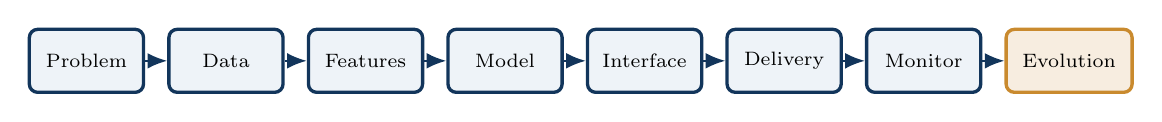
\begin{tikzpicture}[node distance=0.28cm]
  \node[flowbox, minimum width=1.45cm, minimum height=0.8cm] (problem) {\scriptsize Problem};
  \node[flowbox, minimum width=1.45cm, minimum height=0.8cm, right=of problem] (data) {\scriptsize Data};
  \node[flowbox, minimum width=1.45cm, minimum height=0.8cm, right=of data] (features) {\scriptsize Features};
  \node[flowbox, minimum width=1.45cm, minimum height=0.8cm, right=of features] (model) {\scriptsize Model};
  \node[flowbox, minimum width=1.45cm, minimum height=0.8cm, right=of model] (interface) {\scriptsize Interface};
  \node[flowbox, minimum width=1.45cm, minimum height=0.8cm, right=of interface] (delivery) {\scriptsize Delivery};
  \node[flowbox, minimum width=1.45cm, minimum height=0.8cm, right=of delivery] (monitor) {\scriptsize Monitor};
  \node[accentbox, minimum width=1.6cm, minimum height=0.8cm, right=of monitor] (evolution) {\scriptsize Evolution};
  \foreach \a/\b in {problem/data,data/features,features/model,model/interface,interface/delivery,delivery/monitor,monitor/evolution} {
    \draw[arrow] (\a) -- (\b);
  }
  \end{tikzpicture}

  \vspace{0.5em}
  \begin{block}{Today in the course}
  \textbf{Focus:} #1

  \textbf{Bridge:} #2
  \end{block}

  \begin{columns}[T]
  \column{0.48\textwidth}
  \begin{block}{Fraud case}
  {\footnotesize #3}
  \end{block}
  \column{0.48\textwidth}
  \begin{block}{Pasteurization case}
  {\footnotesize #4}
  \end{block}
  \end{columns}

  \vspace{0.3em}
  {\footnotesize \textbf{Course thread:} #5}
  \coursefooter
  \end{frame}
}

\newcommand{\classclosingframe}[4]{
  \begin{frame}{From This Class to the Next}
  \begin{block}{What stays with us}
  #1
  \end{block}

  \begin{columns}[T]
  \column{0.48\textwidth}
  \begin{block}{Project use}
  {\footnotesize #2}
  \end{block}
  \column{0.48\textwidth}
  \begin{block}{Next connection}
  {\footnotesize #3}
  \end{block}
  \end{columns}

  \vspace{0.3em}
  {\footnotesize \textbf{Course thread:} #4}
  \coursefooter
  \end{frame}
}

\tikzset{
  flowbox/.style={
    rounded corners=3pt,
    draw=courseblue,
    fill=courseice,
    very thick,
    minimum width=2.2cm,
    minimum height=0.9cm,
    align=center,
    font=\small
  },
  accentbox/.style={
    rounded corners=3pt,
    draw=coursegold,
    fill=coursegold!15,
    very thick,
    minimum width=2.2cm,
    minimum height=0.9cm,
    align=center,
    font=\small
  },
  arrow/.style={
    -{Latex[length=2.5mm,width=2mm]},
    thick,
    draw=courseblue
  }
}


\title{Class 29: MLOps Practice -- Continuous Training}
\subtitle{Session 29 of 36 -- MLOps Block}
\author{\coursename}
\date{}

\begin{document}

\frame{\titlepage \coursefooter}

\begin{frame}{Agenda}
\begin{itemize}
\item From one-off training to continuous training
\item Triggers for retraining
\item Anatomy of a continuous training pipeline
\item Evaluation gates and champion-challenger promotion
\item Failure modes of automated retraining
\item Practical Component: what exists in this repo today
\end{itemize}
\coursefooter
\end{frame}

\begin{frame}{Training is a pipeline, not an event}
\learninggoals{
\begin{itemize}
\item Explain why manual, ad hoc retraining does not scale past a demo.
\item Identify triggers that should launch a retraining pipeline: schedule, data volume, drift, and performance decay.
\item Describe the stages of a continuous training pipeline and the gates between them.
\item Recognize the difference between automating retraining and automating deployment of a retrained model.
\end{itemize}
}
\coursefooter
\end{frame}

\coursecontextframe
{Operationalizing ML development and training as a repeatable, automatable pipeline.}
{Class 28 introduced MLOps as coordination across the whole lifecycle; this class zooms into one box of that diagram, train and retrain, and asks what it takes to run it without a human kicking it off by hand every time.}
{A continuous training pipeline for fraud scoring would retrain on a schedule or when score drift is detected, then gate promotion on a held-out evaluation before replacing the serving model.}
{A continuous training pipeline for the pasteurization forecaster would retrain as new batches complete, gated by a check that the new model does not regress on known abnormal trajectories.}
{Automation without validation just moves risk faster; a training pipeline needs the same gates as any other release.}

\begin{frame}{From one-off training to continuous training}
\begin{itemize}
\item In a notebook, training is something a person runs once and inspects.
\item In production, the same code needs to run again: new data arrives, labels catch up, or performance decays.
\item Continuous training (CT) means retraining is a repeatable, automatable job, not a manual ritual.
\end{itemize}
\coursefooter
\end{frame}

\begin{frame}{What ``continuous'' means here}
\begin{itemize}
\item Not continuous like a sensor stream: continuous training usually runs on a cadence, not every second.
\item The point is that the pipeline can run unattended and produce a trustworthy candidate model each time.
\item Frequency should match the business reason for retraining, not a fixed habit.
\end{itemize}
\coursefooter
\end{frame}

\begin{frame}{Triggers for retraining}
\begin{tabularx}{\textwidth}{>{\bfseries}l X}
Trigger & When it fires \\
\toprule
Schedule & A fixed cadence, for example nightly or weekly. \\
Data volume & Enough new labeled data has accumulated to justify a refresh. \\
Drift signal & A monitoring alert from Class 31's detectors fires. \\
Performance decay & A tracked metric drops below an agreed threshold. \\
Manual request & A team member has a specific reason to trigger a run. \\
\bottomrule
\end{tabularx}
\coursefooter
\end{frame}

\begin{frame}{Anatomy of a continuous training pipeline}
\centering
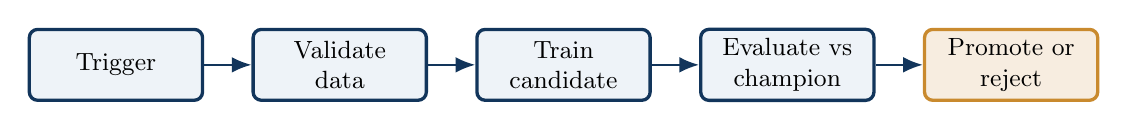
\begin{tikzpicture}[node distance=0.65cm and 0.6cm]
\node[flowbox] (trigger) {Trigger};
\node[flowbox, right=of trigger] (validate) {Validate\\data};
\node[flowbox, right=of validate] (train) {Train\\candidate};
\node[flowbox, right=of train] (eval) {Evaluate vs\\champion};
\node[accentbox, right=of eval] (promote) {Promote or\\reject};
\draw[arrow] (trigger) -- (validate);
\draw[arrow] (validate) -- (train);
\draw[arrow] (train) -- (eval);
\draw[arrow] (eval) -- (promote);
\end{tikzpicture}
\vspace{0.6em}
\begin{itemize}
\item Every arrow is a gate: a candidate that fails a stage should not move forward automatically.
\end{itemize}
\coursefooter
\end{frame}

\begin{frame}{Data validation before training}
\begin{itemize}
\item Schema checks: are the expected columns present, with the expected types?
\item Freshness checks: is the data as recent as the trigger assumed?
\item Volume and balance checks: is there enough signal, and is the label distribution sane?
\item A pipeline that trains on broken data just automates producing a broken model faster.
\end{itemize}
\coursefooter
\end{frame}

\begin{frame}{Evaluation gates before promotion}
\begin{itemize}
\item Compare the new candidate against the current champion on a frozen, held-out evaluation set.
\item Check a business metric, not only a statistical one: review load, false-alert rate, or missed-detection cost.
\item A candidate that wins on one metric but regresses on another needs a human decision, not an automatic merge.
\end{itemize}
\coursefooter
\end{frame}

\begin{frame}{Champion-challenger extends into training}
\begin{itemize}
\item The same champion-challenger idea from monitoring applies to retraining decisions.
\item A newly trained candidate is a challenger until it earns promotion through the evaluation gate.
\item Shadow evaluation on live traffic, before full promotion, catches problems that offline metrics miss.
\end{itemize}
\coursefooter
\end{frame}

\begin{frame}{Where continuous training meets CI/CD}
\begin{itemize}
\item The retraining job itself can be triggered the same way as any other automated workflow: on a schedule or an event.
\item Class 30's GitHub Actions cron trigger is a small but real building block for exactly this kind of scheduled job.
\item Packaging, testing, and versioning from Class 30 apply to the training code path, not only the serving code path.
\end{itemize}
\coursefooter
\end{frame}

\begin{frame}{Failure modes of automated retraining}
\begin{itemize}
\item Feedback loops: a fraud model's own blocking decisions can bias the labels it later retrains on.
\item Drift masking: retraining on recent data can quietly bake in a temporary anomaly as if it were normal.
\item Silent schema drift: an upstream field changes meaning without anyone updating the training code.
\item Unbounded automation: nothing stops a bad candidate from being promoted if a gate is missing or too weak.
\end{itemize}
\begin{block}{Rule}
Every automated stage needs an explicit condition for stopping, not just for proceeding.
\end{block}
\coursefooter
\end{frame}

\begin{frame}{Governance for an automated retraining path}
\begin{itemize}
\item Log every retraining run: trigger reason, data snapshot, metrics, and the promote-or-reject decision.
\item Keep a human approval step for high-stakes promotions, even if triggering is automatic.
\item Version training code and data references together with the resulting model artifact.
\end{itemize}
\coursefooter
\end{frame}

\begin{frame}{Practical Component}
\begin{block}{Honest gap in this repository}
There is currently no automated retraining pipeline in this repository: no scheduled job that pulls new data, retrains, evaluates, and promotes a model.
\end{block}
\begin{itemize}
\item The building blocks exist separately: training code in the notebooks and `streamlit/modeling.py`, and a scheduled-trigger pattern in `tutorials/GitHubActions/tutorial.md`.
\item Wiring them into a real continuous training pipeline is suggested as a separate project, for example a dedicated GitHub submodule, that the course will build going forward.
\item This class stays conceptual on purpose: understand the stages and gates before wiring any automation.
\end{itemize}
\coursefooter
\end{frame}

\begin{frame}{Repo materials we can build on}
\repoactivity{
\begin{itemize}
\item `streamlit/modeling.py` already contains the training and artifact-saving logic a CT pipeline would call.
\item `tutorials/GitHubActions/tutorial.md`'s cron-triggered workflow is the closest existing building block for a scheduled retraining job.
\item Neither piece is wired to the other yet; that gap is exactly what a continuous training project would close.
\end{itemize}
}
\coursefooter
\end{frame}

\begin{frame}{Discussion prompt}
\begin{block}{Question}
If a retraining pipeline ran fully unattended, which single gate would you refuse to automate away, and why?
\end{block}
\begin{itemize}
\item This forces a concrete stance on where human judgment stays load-bearing.
\item It also previews the governance theme that returns in later monitoring and scaling discussions.
\end{itemize}
\coursefooter
\end{frame}

\begin{frame}{Papers and materials}
\readinglist{
\href{https://www.oreilly.com/library/view/designing-machine-learning/9781098107956/}{Chip Huyen, Designing Machine Learning Systems};\
\href{https://cloud.google.com/architecture/mlops-continuous-delivery-and-automation-pipelines-in-machine-learning}{Google Cloud MLOps guidance on CI/CD/CT for ML};\
\href{https://research.google/pubs/pub46555/}{Sculley et al., Hidden Technical Debt in Machine Learning Systems};\
\href{https://www.oreilly.com/library/view/practical-mlops/9781098103002/}{Practical MLOps}.
}
\coursefooter
\end{frame}

\classclosingframe
{\begin{itemize}
\item Continuous training turns retraining from a manual ritual into a governed, repeatable pipeline.
\item Triggers, data validation, evaluation gates, and promotion decisions all need explicit rules.
\item Automating a bad process just produces bad models faster; the gates matter more than the automation.
\end{itemize}}
{Teams should now be able to describe, even without building it, what a retraining pipeline for their own project would trigger on and what would stop a bad candidate.}
{Class 30 returns to the delivery side of the pipeline: Docker and GitHub Actions for packaging and shipping what Class 28 and Class 29 have described.}
{Training and delivery are two automatable paths that both need the same discipline: gates, versioning, and observability.}

\end{document}
